\documentclass{article}
\usepackage[utf8]{vietnam}
\usepackage{amsmath}
\usepackage{graphicx}
\graphicspath{ {./image/} }\usepackage{hyperref}
\title{TRUYEN SO LIEU VA MANG}

\begin{document}

Từ mã của các nodes: 
\begin{itemize}
\item F: 000
\item E: 001
\item A: 01
\item D: 100
\item C: 101
\item H: 11000
\item I: 11001
\item J: 110100
\item K: 110101
\item G: 11011
\item B: 111
\end{itemize}
Entropy:
\[
\sum_{i=0}^{k} \frac{\log{\left(\frac{1}{{p}_{i}} \right)} {p}_{i}}{\log{\left(2 \right)}} = 3.11
\]
Chiều dài TB từ mã:
\[
N = \sum_{i=0}^{k} {N}_{i} {p}_{i} = 3.15
\]
Hiệu suất Huffman:
\[
\frac{H}{N} = 0.987
\]
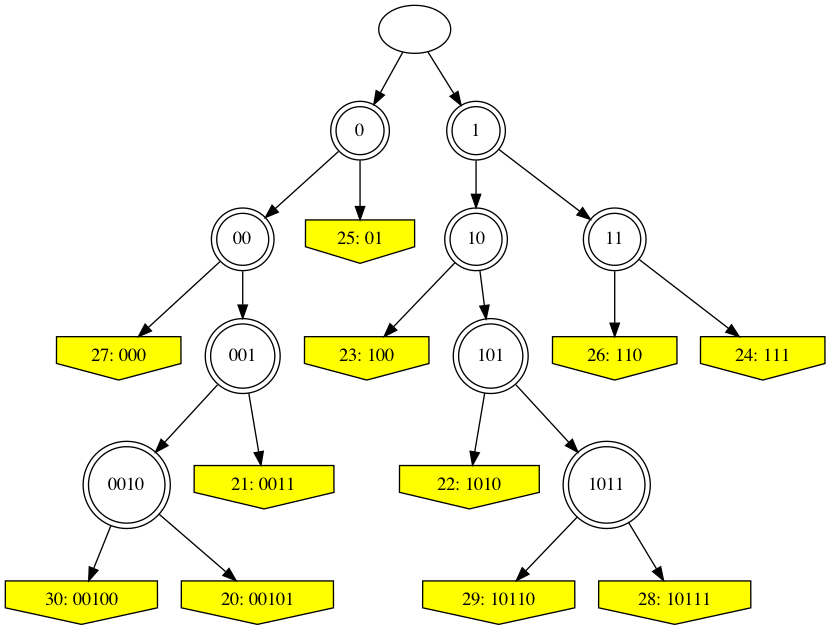
\includegraphics[width=\textwidth]{graph.png}
\begin{center}
\textit{Hình 1. Cây Huffman}
\end{center}
\end{document}
